\chapter{Code, Class, and Master Data Schema for Coffee Chain ERP System}

\section*{Introduction}
This chapter explains the master data structure and schema used in the Coffee Chain ERP system. It first introduces key terminologies for understanding ERP data models, then describes the master data entities, relationships, and schema as implemented in the system. This provides a foundation for understanding the system’s code and database structure.

\section*{Basic Terminologies}

\begin{description}
    \item[Entity:] A distinct object or concept in the system that stores data. Examples include Customer, Product, or Outlet.
    \item[Attribute:] A property or field of an entity. For example, a Customer entity may have attributes such as Name, Email, and Phone Number.
    \item[Primary Key:] A unique identifier for an entity instance. In Odoo, this is often the \texttt{id} field.
    \item[Relationship:] The association between two entities, such as One-to-Many or Many-to-One. Example: Each Outlet is owned by one Outlet Owner, while an owner can have multiple outlets.
    \item[Master Data:] Core data that is essential for the operation of a system, such as Customers, Products, and Outlets.
    \item[Business Logic Layer:] Code that defines the rules and behavior of the system, often implemented via Python classes in Odoo modules.
    \item[Model/Class:] In Odoo, a model is a Python class that defines the structure of an entity, including fields, relationships, and methods.
\end{description}

\section*{Master Data in Coffee Chain ERP System}
The Coffee Chain ERP system’s master data schema includes the following key entities:

\subsection*{Outlet Owner (\texttt{res.partner})}
\begin{tabular}{|l|l|l|}
\hline
\textbf{Field} & \textbf{Type} & \textbf{Description} \\
\hline
id & int & Primary Key \\
name & string & Owner Name \\
email & string & Contact Email \\
phone & string & Contact Number \\
\hline
\end{tabular}

\noindent
\textbf{Relationship:} One owner can manage multiple Coffee Outlets (One-to-Many).

\subsection*{Coffee Outlet (\texttt{coffee.outlet})}
\begin{tabular}{|l|l|l|l|}
\hline
\textbf{Field} & \textbf{Type} & \textbf{Description} & \textbf{Relationship} \\
\hline
id & int & Primary Key & — \\
name & string & Outlet Name & — \\
location & string & Outlet Address & — \\
owner\_id & int & Foreign Key & res.partner.id (Outlet Owner) \\
\hline
\end{tabular}

\noindent
\textbf{Relationships:} Many-to-One with Outlet Owner, One-to-Many with Sale Orders.

\subsection*{Coffee Menu Item (\texttt{coffee.menu.item})}
\begin{tabular}{|l|l|l|}
\hline
\textbf{Field} & \textbf{Type} & \textbf{Description} \\
\hline
id & int & Primary Key \\
name & string & Item Name \\
price & float & Item Price \\
category & selection & Drinks / Snacks \\
image & binary & Item Image \\
\hline
\end{tabular}

\noindent
\textbf{Relationship:} Many-to-Many with Sale Orders.

\subsection*{Sale Customer (\texttt{res.partner})}
\begin{tabular}{|l|l|l|}
\hline
\textbf{Field} & \textbf{Type} & \textbf{Description} \\
\hline
id & int & Primary Key \\
name & string & Customer Name \\
email & string & Contact Email \\
phone & string & Contact Number \\
\hline
\end{tabular}

\noindent
\textbf{Relationship:} One-to-Many with Sale Orders; optional link to CRM Leads.

\subsection*{Sale Order (\texttt{sale.order})}
\begin{tabular}{|l|l|l|l|}
\hline
\textbf{Field} & \textbf{Type} & \textbf{Description} & \textbf{Relationship} \\
\hline
id & int & Primary Key & — \\
order\_number & string & Unique Order Number & --- \\
customer\_id & int & Foreign Key & res.partner.id (Sale Customer) \\
outlet\_id & int & Foreign Key & coffee.outlet.id \\
order\_date & date & Order Timestamp & --- \\
\hline
\end{tabular}

\noindent
\textbf{Relationship:} Many-to-One with Sale Customer and Outlet; Many-to-Many with Menu Items; optional FK to CRM Lead.

\subsection*{CRM Lead (\texttt{crm.lead})}
\begin{tabular}{|l|l|l|l|}
\hline
\textbf{Field} & \textbf{Type} & \textbf{Description} & \textbf{Relationship} \\
\hline
id & int & Primary Key & — \\
lead\_name & string & Lead Title & --- \\
stage & string & Lead Status & — \\
related\_order\_id & int & Optional FK & sale.order.id \\
\hline
\end{tabular}

\noindent
\textbf{Relationship:} Optional linkage to Sale Orders and Sale Customers.

\section*{Master Data Schema Diagram}
The following diagram visually represents the **tables, fields, primary keys, and relationships** in the Coffee Chain ERP system:

%\begin{figure}[H]
 %   \centering
  %  \includegraphics[width=0.9\textwidth]{diagrams/masterdata_schema.png}
   % \caption{Master Data Schema showing entities, attributes, primary keys, and relationships.}
%\end{figure}

\section*{Python Classes Mapping to Master Data}
The ERP system implements the master data entities as Python classes in Odoo modules:

\begin{itemize}
    \item \texttt{coffee.outlet} → Python class \texttt{CoffeeOutlet(models.Model)}
    \item \texttt{coffee.menu.item} → Python class \texttt{CoffeeMenuItem(models.Model)}
    \item \texttt{res.partner} → Used for both Outlet Owner and Sale Customer
    \item \texttt{sale.order} → Python class \texttt{SaleOrder(models.Model)}
    \item \texttt{crm.lead} → Python class \texttt{CrmLead(models.Model)}
\end{itemize}

\subsection*{Field Definitions Example}
For example, the \texttt{CoffeeMenuItem} class defines the following fields:

\begin{lstlisting}[language=Python, caption={Coffee Menu Item Python Class}]
from odoo import models, fields

class CoffeeMenuItem(models.Model):
    _name = 'coffee.menu.item'
    _description = 'Coffee Menu Item'

    name = fields.Char(required=True)
    price = fields.Monetary(currency_field='currency_id', required=True)
    category = fields.Selection([
        ('drinks', 'Drinks'),
        ('snacks', 'Snacks'),
    ], required=True)
    image = fields.Image(max_width=128, max_height=128)
\end{lstlisting}

\begin{figure}[H]
    \centering
    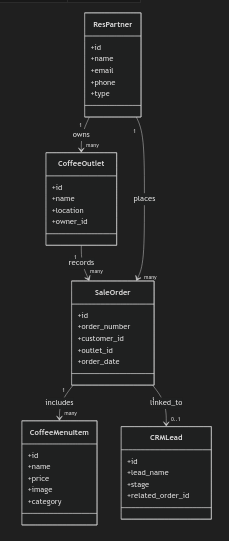
\includegraphics[width=0.356\textwidth]{diagrams/masterdata.png}
    \caption{Class diagram showing Python classes and field names for quick reference.}
\end{figure}

\section*{Summary}
The master data schema of the Coffee Chain ERP system ensures:

\begin{itemize}
    \item Clear separation of entities: outlets, menu items, customers, orders, and leads.
    \item Proper relationships to maintain data integrity: e.g., orders linked to customers and outlets.
    \item Python classes in Odoo accurately define the structure, fields, and relationships.
    \item The schema supports the business logic and workflow described in previous chapters.
\end{itemize}
